\documentclass[a4paper ]{article}
\usepackage{graphicx}
\usepackage[letterpaper, landscape, margin=2in]{geometry}
\geometry{
	paper=a4paper, % Change to letterpaper for US letter
	inner=0.5cm, % Inner margin
	outer=0.5cm, % Outer margin
	bindingoffset=0.01cm, % Binding offset
	top=0.5cm, % Top margin
	bottom=0.5cm, % Bottom margin
	%showframe, % Uncomment to show how the type block is set on the page
}
\usepackage[utf8]{inputenc}
%\usepackage{natbib}

\begin{document}
- - -

\vspace{50mm}
\begin{center}
{\Huge \textsc{\textbf{Modelos Delta:}}}\\
{\Huge \textsc{\textbf{Estimando el tamaño de la diferencia entre d'(A) y d'(B)}}}\\
\vspace{20mm}
\end{center}

\begin{center}
\textit{\huge Estudios en Detección de Señales - Tesis de Licenciatura}\\
\bigskip
\end{center}

\begin{center}
\textit{\huge Adriana F. Chávez De la Peña}\\
\end{center}

\begin{center}
\vfill
\textit{\huge adrifelcha@gmail.com}\\
\end{center}

\newpage




---
\vspace{3mm}
\begin{center}
{\LARGE \textbf{Modelo gráfico 1:} C y D son jerárquicos}\\
{\small \textsc{(El parámetro delta estima las diferencias entre d'(A) y d'(B))}}\\
\smallskip
\end{center}

\vspace{3mm}
\begin{figure}[th]
\centering
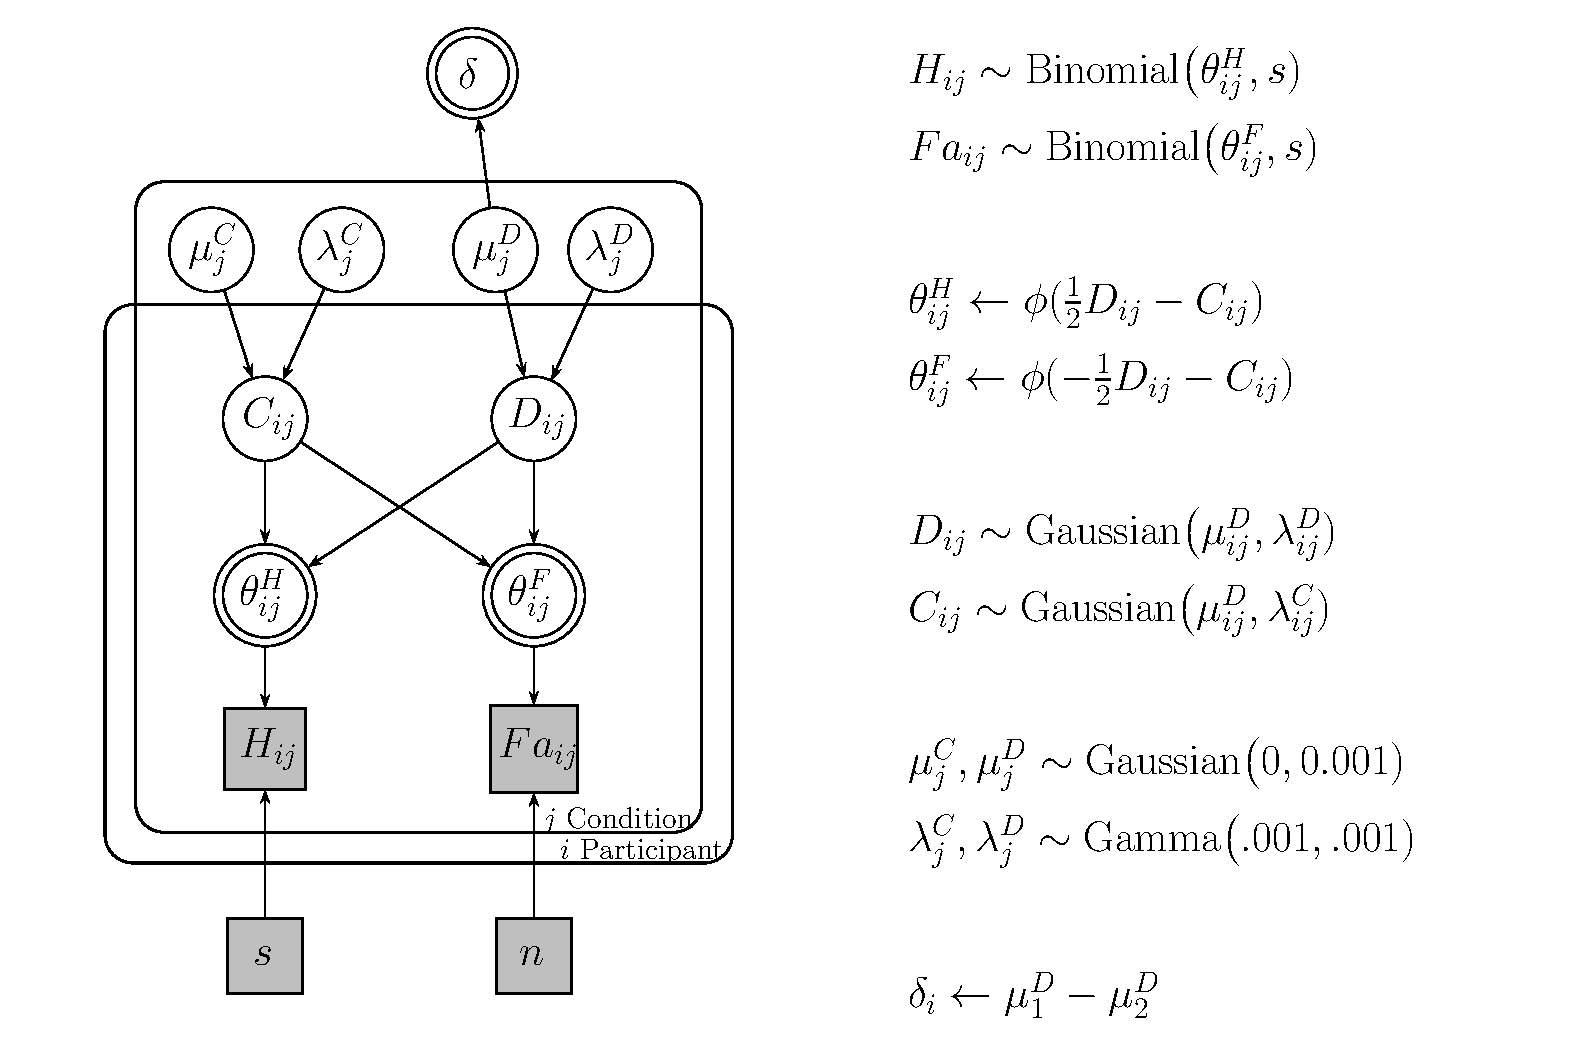
\includegraphics[width=.8\textwidth]{Figures/Delta_EP_CyDHierarchichal}
\end{figure}
\clearpage



---
\vspace{3mm}
\begin{center}
{\LARGE \textbf{Modelo gráfico 2:} Sólo D es jerárquicos}\\
{\small \textsc{(El parámetro delta estima las diferencias entre d'(A) y d'(B))}}\\
\smallskip
\end{center}

\vspace{3mm}
\begin{figure}[th]
\centering
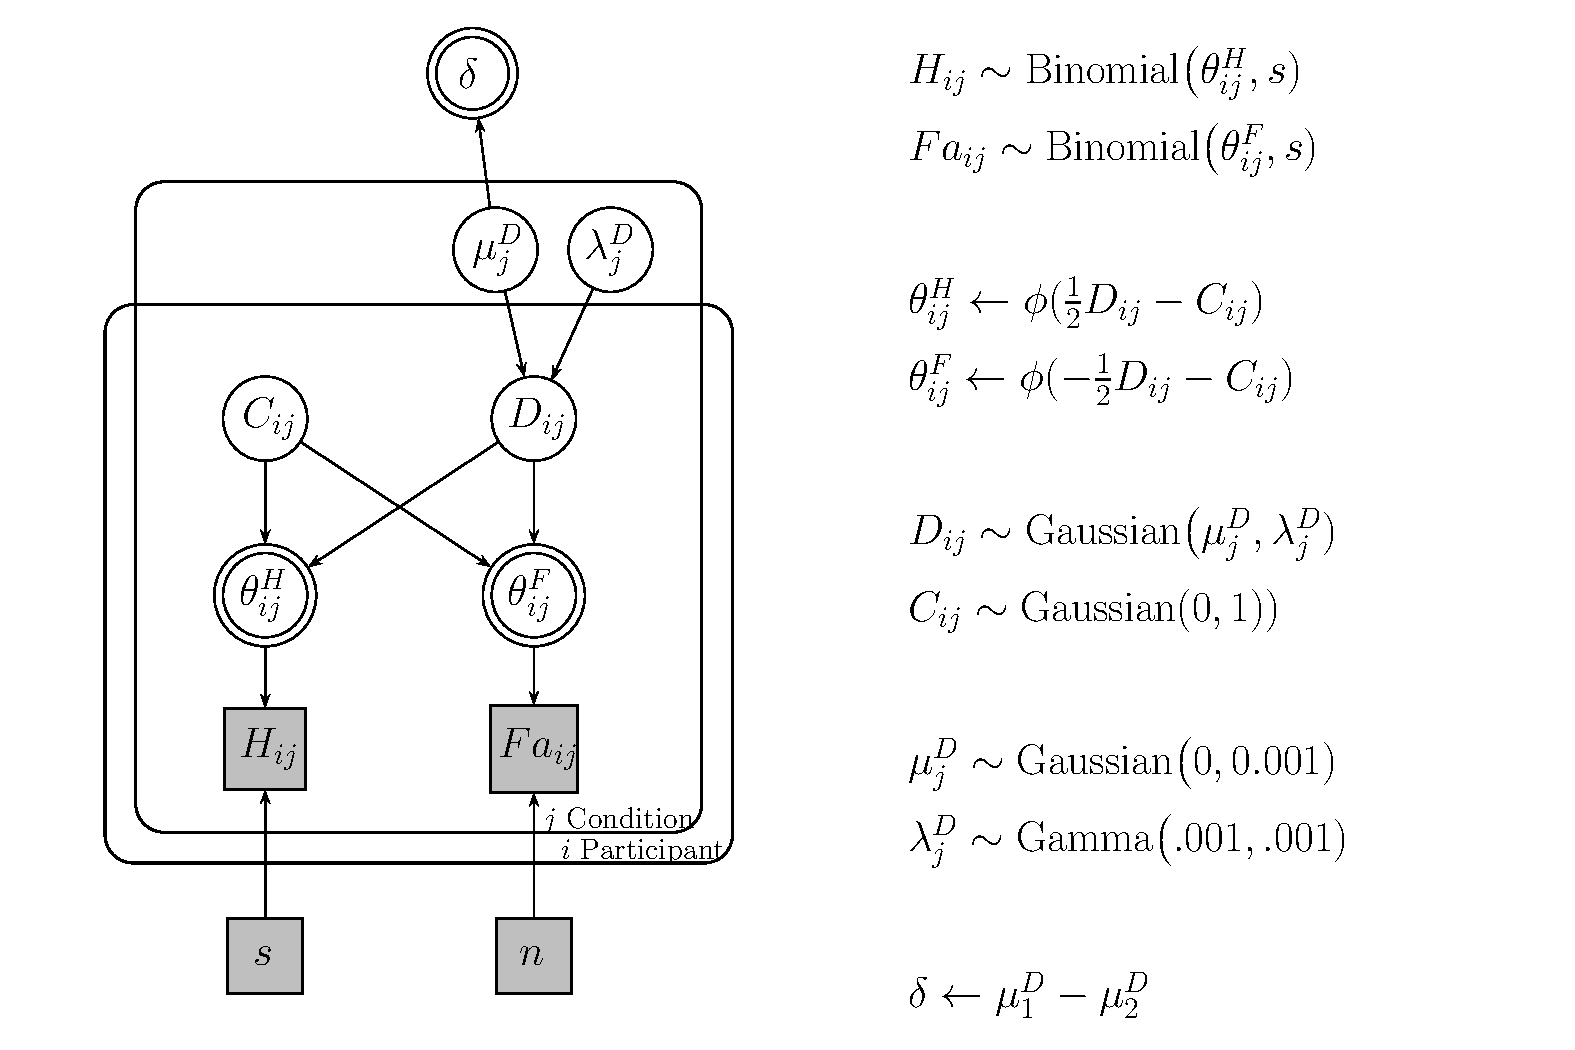
\includegraphics[width=.8\textwidth]{Figures/Delta_EP_DHierarchichal}
\end{figure}
\clearpage


---
\vspace{3mm}
\begin{center}
{\LARGE \textbf{Modelo gráfico 4:} D es jerárquico y sólo hay una C.}\\
{\small \textsc{(El parámetro delta estima las diferencias entre d'(A) y d'(B))}}\\
\smallskip
\end{center}

\vspace{3mm}
\begin{figure}[th]
\centering
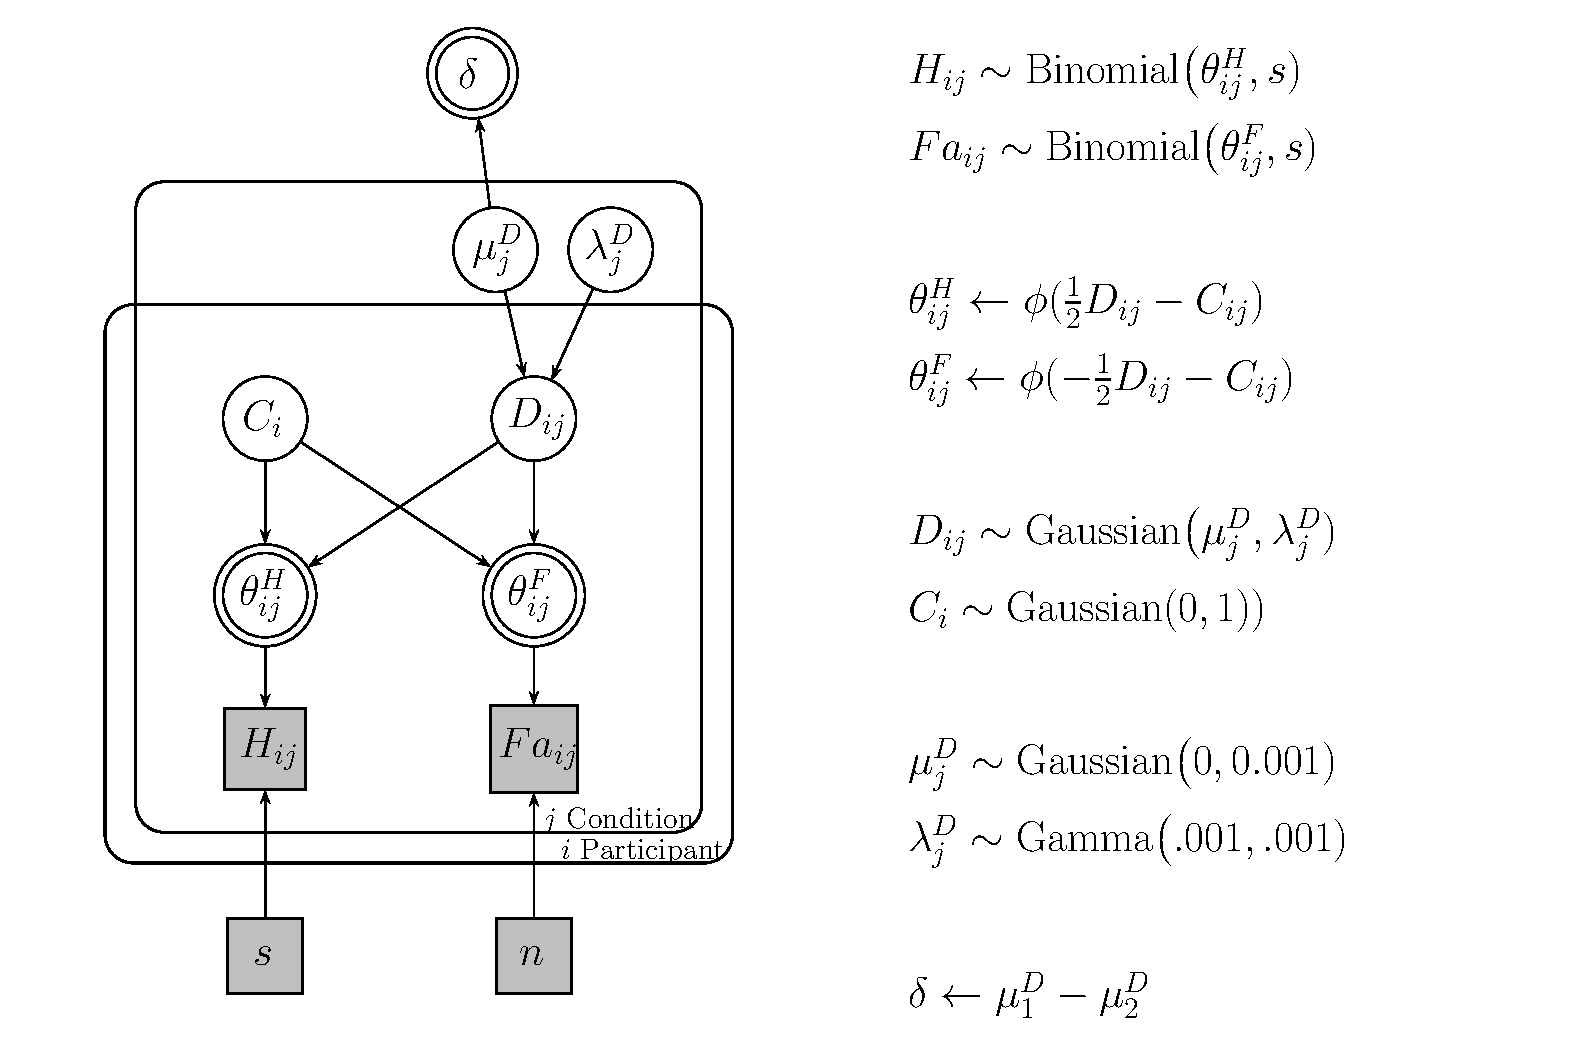
\includegraphics[width=.8\textwidth]{Figures/Delta_EP_DHierarchichal_SingleC}
\end{figure}
\clearpage





---
\vspace{3mm}
\begin{center}
{\LARGE \textbf{Modelo gráfico 4:} Sólo hay una C y también es jerárquica.}\\
{\small \textsc{(El parámetro delta estima las diferencias entre d'(A) y d'(B))}}\\
\smallskip
\end{center}

\vspace{3mm}
\begin{figure}[th]
\centering
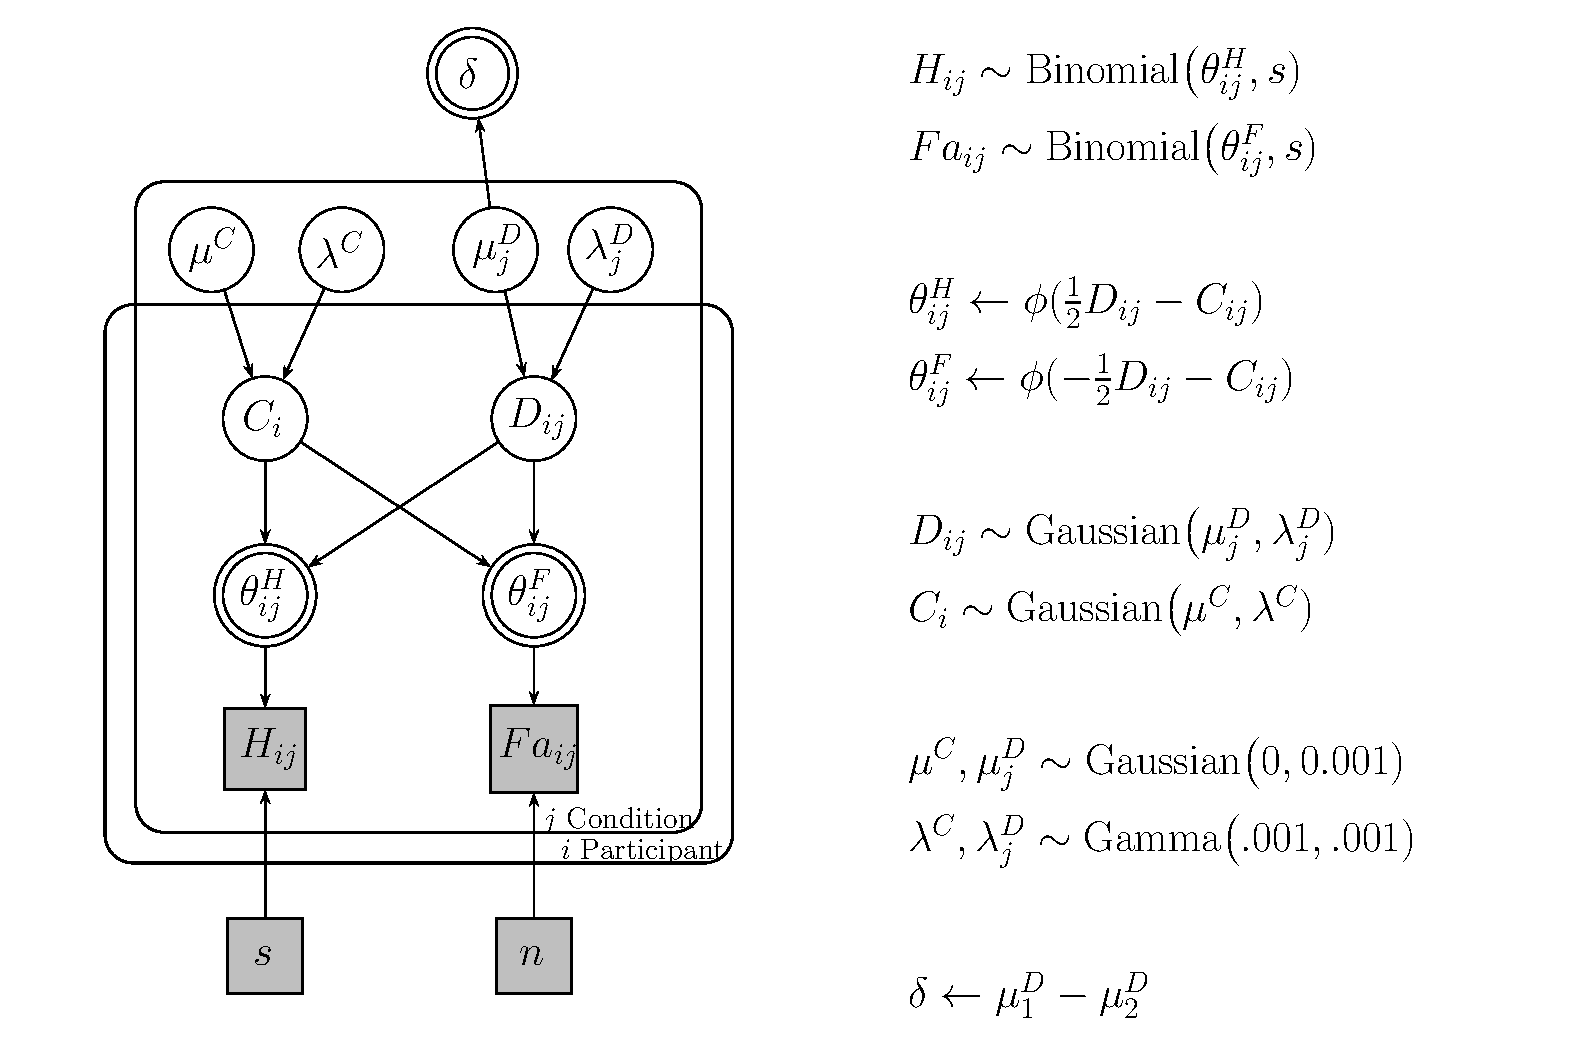
\includegraphics[width=.8\textwidth]{Figures/Delta_EP_CyDHierarchical_SingleC}
\end{figure}
\clearpage





\end{document}